\documentclass[11pt]{article}

\usepackage[a4paper,margin=2.4cm]{geometry}
\usepackage[T1]{fontenc}
\usepackage[utf8]{inputenc}
\usepackage{amsmath,amssymb}
\usepackage{xcolor}
\usepackage{tcolorbox}
\usepackage{tikz}
\usepackage{booktabs}
\usepackage{enumitem}
\usepackage{titlesec}
\usepackage{fancyhdr}
\usepackage{hyperref}
\usetikzlibrary{arrows.meta, positioning, fit, backgrounds}
\tcbuselibrary{skins,breakable}

% ---------- paleta ----------
\definecolor{navy}{HTML}{0B132B}
\definecolor{teal}{HTML}{1C7C74}
\definecolor{amber}{HTML}{D98E2B}
\definecolor{red}{HTML}{C1443C}
\definecolor{paper}{HTML}{FBFAF7}
\definecolor{inkgray}{HTML}{3A3A3A}

\pagecolor{paper}
\color{inkgray}

% ---------- títulos ----------
\titleformat{\section}
  {\normalfont\Large\bfseries\color{navy}}
  {\thesection}{0.6em}{}
\titleformat{\subsection}
  {\normalfont\large\bfseries\color{teal}}
  {\thesubsection}{0.6em}{}

\pagestyle{fancy}
\fancyhf{}
\renewcommand{\headrulewidth}{0.4pt}
\fancyhead[L]{\small\color{navy}\textsc{Do score ao erro}}
\fancyhead[R]{\small\color{navy}Prof. Thiago M. Paixão}
\fancyfoot[C]{\small\thepage}

\hypersetup{colorlinks=true, linkcolor=teal, urlcolor=teal}

% ---------- caixas de destaque ----------
\newtcolorbox{intuicao}{
  breakable, enhanced, colback=teal!6, colframe=teal,
  boxrule=0.6pt, arc=2pt, left=8pt, right=8pt, top=6pt, bottom=6pt,
  title={\textbf{\small \textbullet\ INTUIÇÃO}}, coltitle=white,
  colbacktitle=teal, fonttitle=\small, boxsep=2pt
}

\newtcolorbox{checagem}{
  breakable, enhanced, colback=amber!8, colframe=amber,
  boxrule=0.6pt, arc=2pt, left=8pt, right=8pt, top=6pt, bottom=6pt,
  title={\textbf{\small \textbullet\ CHECAGEM DE SANIDADE}}, coltitle=white,
  colbacktitle=amber!90!black, fonttitle=\small, boxsep=2pt
}

\newtcolorbox{resultado}{
  breakable, enhanced, colback=navy!5, colframe=navy,
  boxrule=0.8pt, arc=2pt, left=8pt, right=8pt, top=6pt, bottom=6pt,
}

\newtcolorbox{curiosos}{
  breakable, enhanced, colback=paper, colframe=inkgray!60,
  boxrule=0.6pt, arc=2pt, left=9pt, right=9pt, top=7pt, bottom=7pt,
  borderline west={2.4pt}{0pt}{amber},
  title={\textbf{\small \textbullet\ PARA OS CURIOSOS --- de onde vem essa fórmula}},
  coltitle=navy, colbacktitle=paper, fonttitle=\small,
  boxsep=2pt
}

\newcommand{\scoreb}[1]{\textcolor{teal}{#1}}
\newcommand{\errb}[1]{\textcolor{red}{#1}}

\title{}
\date{}

\begin{document}

% ---------------- CAPA / INTRO ----------------
\begin{center}
  {\Huge\bfseries\color{navy} Do Score ao Erro}\\[4pt]
  {\Large\color{teal} Softmax, Perda e Gradientes --- um guia intuitivo}\\[10pt]
  {\small Prof. Thiago M. Paixão \quad$\cdot$\quad Ifes --- Campus Serra}
\end{center}

\vspace{0.4cm}
\noindent
Pense num sistema de \emph{ranking} qualquer --- um placar de partida, um retorno de API que atribui uma pontuação a cada opção. É basicamente isso que uma rede neural de classificação faz na última camada: para cada classe possível, ela calcula um \textbf{score} (chamado de \emph{logit}). Só que scores brutos não são probabilidades --- podem ser negativos, não somam 1, não são comparáveis entre si de forma direta. Esta nota constrói, passo a passo, a ``tubulação'' que transforma esses scores em probabilidades e, a partir delas, em um sinal de erro que a rede usa para aprender.

\vspace{0.2cm}
\noindent Vamos do caso mais simples (um único exemplo) até a forma que você de fato escreve em código (mini-batches vetorizados) --- e, no caminho, vamos abrir o capô e calcular os gradientes manualmente, sem atalhos, para que a mágica do \texttt{loss.backward()} pare de ser mágica.

\bigskip
\noindent\rule{\textwidth}{0.4pt}

% ---------------- SEÇÃO 1 ----------------
\section{Um único exemplo}

Seja $x \in \mathbb{R}^d$ um vetor de entrada (por exemplo, os pixels de uma imagem já achatados em um vetor) e $C$ o número de classes. Cada classe $k$ tem seu próprio ``detector de score'': um vetor de pesos $w_k \in \mathbb{R}^d$ e um viés escalar $b_k$.

$$
W = \begin{bmatrix} w_1 \\ \vdots \\ w_C \end{bmatrix} \in \mathbb{R}^{C\times d}, \qquad
b = \begin{bmatrix} b_1 \\ \vdots \\ b_C \end{bmatrix} \in \mathbb{R}^{C}
$$

\subsection*{Passo 1 --- Scores (logits)}

$$
z_k = w_k^\top x + b_k, \qquad k = 1, \dots, C
$$

Cada $z_k$ mede o quanto a entrada $x$ ``se parece'' com a classe $k$, segundo os pesos atuais. É um número real qualquer --- pode ser $-8.3$, pode ser $52.1$. Ainda não é probabilidade.

\begin{intuicao}
Pense em $w_k$ como um ``molde'' aprendido para a classe $k$. O produto $w_k^\top x$ é literalmente uma medida de similaridade (produto interno) entre a entrada e esse molde: quanto mais $x$ se alinha com $w_k$, maior o score $z_k$.
\end{intuicao}

\subsection*{Passo 2 --- Softmax: de scores a probabilidades}

$$
p_k = \operatorname{softmax}(z)_k = \frac{e^{z_k}}{\sum_{j=1}^{C} e^{z_j}}
$$

O softmax faz três coisas ao mesmo tempo: (i) exponencia cada score, tornando tudo positivo; (ii) normaliza pela soma, garantindo $\sum_k p_k = 1$; (iii) \emph{exagera} as diferenças relativas --- um score um pouco maior que os outros vira uma probabilidade proporcionalmente muito maior, graças à exponencial.

\begin{intuicao}
É como transformar os pontos de um campeonato em ``probabilidade de título''. Não basta ter mais pontos que o adversário: o quanto \emph{a mais} importa, e o softmax captura exatamente essa não linearidade.
\end{intuicao}

\subsection*{Passo 3 --- A perda: penalizando a probabilidade errada}

Se $y$ é a classe correta do exemplo, a perda de entropia cruzada é:

$$
\mathcal{L} = -\log(p_y)
$$

\begin{intuicao}
$-\log(\cdot)$ é uma função que vale $0$ quando o argumento é $1$, e explode para $+\infty$ quando o argumento tende a $0$. Ou seja: se o modelo acerta com $p_y \approx 1$, a perda é quase nula (\emph{sem} castigo). Se o modelo erra feio, com $p_y \approx 0$ (achava que a classe correta era quase impossível), a perda dispara. É um professor rigoroso: só reclama quando você erra, e reclama \emph{muito mais} quanto mais confiante você estava no erro.
\end{intuicao}

\begin{center}
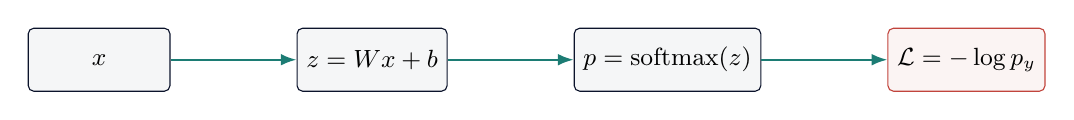
\begin{tikzpicture}[
  node distance=13mm and 16mm,
  box/.style={draw=navy, rounded corners=2pt, fill=navy!4, minimum height=8mm, minimum width=18mm, align=center, font=\small},
  arr/.style={-{Latex[length=2mm]}, thick, teal}
]
  \node[box] (x) {$x$};
  \node[box, right=of x] (z) {$z = Wx+b$};
  \node[box, right=of z] (p) {$p=\operatorname{softmax}(z)$};
  \node[box, right=of p, fill=red!6, draw=red] (L) {$\mathcal{L}=-\log p_y$};

  \draw[arr] (x) -- (z);
  \draw[arr] (z) -- (p);
  \draw[arr] (p) -- (L);
\end{tikzpicture}
\end{center}

\noindent Note que a perda depende de \textbf{todos} os $z_j$ (via o denominador do softmax), não apenas de $z_y$ --- isso vai importar na hora de derivar.

% ---------------- SEÇÃO 2 ----------------
\section{Do exemplo para o dataset inteiro}

Com $N$ exemplos $\{(x^{(i)}, y^{(i)})\}_{i=1}^N$, cada um passa pela \emph{mesma} tubulação (mesmos $W,b$, compartilhados), gerando seu próprio $z^{(i)}$, $p^{(i)}$ e perda individual $-\log\!\big(p^{(i)}_{y^{(i)}}\big)$.

A perda do dataset é simplesmente a \textbf{média} das perdas individuais:

$$
\mathcal{L}(W,b) = \frac{1}{N}\sum_{i=1}^{N} -\log\!\left(p^{(i)}_{y^{(i)}}\right)
$$

\begin{intuicao}
$W$ e $b$ são os únicos ``botões'' que o treinamento pode girar --- e eles são \textbf{compartilhados} por todos os $N$ exemplos. Treinar é encontrar os valores de $W,b$ que, em média, deixam o time (todos os exemplos) satisfeito, não apenas um exemplo específico.
\end{intuicao}

% ---------------- SEÇÃO 3 ----------------
\section{Do dataset para o mini-batch}

Calcular $\mathcal{L}$ sobre os $N$ exemplos a cada passo de treino é caro (imagine $N=1{,}2$ milhão de imagens). Na prática, sorteia-se um subconjunto pequeno $\mathcal{B} \subset \{1,\dots,N\}$, de tamanho $B=|\mathcal{B}|$ (tipicamente $32$, $64$, $128$\dots), a cada iteração:

$$
\mathcal{L}_{\mathcal{B}}(W,b) = \frac{1}{B}\sum_{i \in \mathcal{B}} -\log\!\left(p^{(i)}_{y^{(i)}}\right)
$$

\begin{intuicao}
$\mathcal{L}_\mathcal{B}$ é uma amostra aleatória de $\mathcal{L}$ --- como perguntar a $B$ pessoas escolhidas ao acaso, em vez da população inteira, para estimar uma opinião média. Não é exato, mas é um estimador \emph{não enviesado} ($\mathbb{E}[\mathcal{L}_\mathcal{B}] = \mathcal{L}$) e muitíssimo mais barato de calcular. É essa troca --- precisão por velocidade --- que viabiliza o treinamento de redes grandes (SGD, Adam, etc.).
\end{intuicao}

\bigskip
\noindent\rule{\textwidth}{0.4pt}
\bigskip

\begin{center}
{\Large\bfseries\color{navy} Parte II --- Abrindo o capô: os gradientes}
\end{center}
\bigskip

Agora a pergunta que interessa para o treino: \emph{em que direção devo mexer cada peso para diminuir a perda?} Essa direção é o gradiente. Vamos calculá-lo primeiro ``na mão'', coordenada a coordenada --- e só depois compactar tudo em notação matricial.

% ---------------- SEÇÃO 4 ----------------
\section{Gradiente --- versão não vetorizada}

Queremos $\dfrac{\partial \mathcal{L}}{\partial w_k}$ e $\dfrac{\partial \mathcal{L}}{\partial b_k}$, para cada classe $k=1,\dots,C$, ainda para um único exemplo.

\subsection*{Passo 1 --- gradiente em relação ao score $z_k$}

Aplicando a regra da cadeia através do softmax e do $-\log$, chega-se a um resultado surpreendentemente limpo:

\begin{resultado}
$$
\frac{\partial \mathcal{L}}{\partial z_k} = p_k - \mathbf{1}[k=y]
$$
\end{resultado}

onde $\mathbf{1}[k=y]$ vale $1$ se $k$ é a classe correta, e $0$ caso contrário.

\begin{curiosos}
O truque é reescrever $\mathcal{L}$ de um jeito que "abra" o softmax em vez de escondê-lo dentro de uma fração. Denotando $S = \sum_{j=1}^{C} e^{z_j}$ (a soma no denominador do softmax, de modo que $p_j = e^{z_j}/S$):

$$
\mathcal{L} = -\log(p_y) = -\log\!\left(\frac{e^{z_y}}{S}\right) = -\log\big(e^{z_y}\big) + \log(S) = -z_y + \log(S)
$$

(usamos a propriedade $\log(a/b) = \log a - \log b$, e $\log(e^{z_y}) = z_y$). Agora $\mathcal{L}$ é uma soma de dois termos bem mais simples de derivar: um termo linear ($-z_y$) e um termo que só depende de $S$.

\medskip
\noindent\textbf{Derivando o primeiro termo, $-z_y$, em relação a $z_k$:}

$z_y$ é apenas \emph{uma} das coordenadas do vetor $z$ --- a da classe correta. Derivar $z_y$ em relação a $z_k$ só dá algo diferente de zero quando $k$ é exatamente essa coordenada:

$$
\frac{\partial(-z_y)}{\partial z_k} = -\mathbf{1}[k=y]
$$

\medskip
\noindent\textbf{Derivando o segundo termo, $\log(S)$, em relação a $z_k$:}

Aqui usamos a regra da cadeia ($\frac{d}{du}\log(u) = \frac{1}{u}\cdot\frac{du}{dz_k}$) com $u=S$:

$$
\frac{\partial \log(S)}{\partial z_k} = \frac{1}{S}\cdot\frac{\partial S}{\partial z_k}
$$

Como $S = \sum_{j=1}^{C} e^{z_j}$, e apenas o termo $j=k$ dessa soma depende de $z_k$:

$$
\frac{\partial S}{\partial z_k} = \frac{\partial}{\partial z_k}\sum_{j=1}^{C} e^{z_j} = e^{z_k}
$$

Substituindo de volta:

$$
\frac{\partial \log(S)}{\partial z_k} = \frac{e^{z_k}}{S} = p_k
$$

(a última igualdade é só a própria definição de softmax --- $p_k = e^{z_k}/S$.)

\medskip
\noindent\textbf{Somando os dois termos:}

$$
\frac{\partial \mathcal{L}}{\partial z_k} = \underbrace{-\mathbf{1}[k=y]}_{\text{do termo } -z_y} \;+\; \underbrace{p_k}_{\text{do termo } \log(S)} = p_k - \mathbf{1}[k=y]
$$

Repare que \emph{não} precisamos separar ``na mão'' os casos $k=y$ e $k\neq y$ --- o indicador $\mathbf{1}[k=y]$ já nasce naturalmente da derivada de $z_y$ e carrega essa distinção sozinho. Mas, para conferir, vale substituir os dois casos:

\begin{itemize}[leftmargin=1.4em]
  \item Se $k=y$: $\;\partial\mathcal{L}/\partial z_k = p_y - 1$ (negativo, pois $p_y\le 1$).
  \item Se $k\neq y$: $\;\partial\mathcal{L}/\partial z_k = p_k - 0 = p_k$ (positivo, pois $p_k \ge 0$).
\end{itemize}

exatamente os dois comportamentos discutidos na caixa de intuição acima.
\end{curiosos}

\begin{intuicao}
Esse termo é literalmente o ``erro'' de cada score: a diferença entre o que o modelo \emph{previu} ($p_k$) e o que \emph{deveria} ter previsto ($1$ para a classe certa, $0$ para as demais). Se o modelo acerta perfeitamente ($p_y=1$, $p_{k\neq y}=0$), esse erro é zero em todas as coordenadas --- e o gradiente desaparece, sinalizando ``nada a corrigir aqui''.
\end{intuicao}

\subsection*{Passo 2 --- propagando até $w_k$ e $b_k$}

Como $z_k = w_k^\top x + b_k$, temos $\dfrac{\partial z_k}{\partial w_k} = x$ e $\dfrac{\partial z_k}{\partial b_k}=1$. Pela regra da cadeia:

\begin{resultado}
$$
\frac{\partial \mathcal{L}}{\partial w_k} = \big(p_k - \mathbf{1}[k=y]\big)\, x
\qquad\qquad
\frac{\partial \mathcal{L}}{\partial b_k} = p_k - \mathbf{1}[k=y]
$$
\end{resultado}

\begin{intuicao}
\textbf{Se $k$ é a classe correta} ($k=y$): o gradiente é $(p_y-1)x$, e como $p_y \le 1$ esse fator é $\le 0$. O passo de descida do gradiente (que \emph{subtrai} o gradiente) vai então \emph{aumentar} $w_y^\top x$ --- empurrando $p_y$ para mais perto de $1$. Faz sentido: queremos reforçar a classe certa.

\textbf{Se $k$ é uma classe errada} ($k\neq y$): o gradiente é $p_k \cdot x$, positivo. O passo de descida vai \emph{diminuir} $w_k^\top x$ --- suprimindo a confiança nas classes erradas. O modelo está literalmente ``roubando'' probabilidade das classes erradas para dar à classe certa.
\end{intuicao}

% ---------------- SEÇÃO 5 ----------------
\section{Forma vetorizada}

Empilhar $C$ equações escalares repetidas é sinal de que dá para escrever em forma vetorial. Defina o \textbf{vetor de erro} $\delta \in \mathbb{R}^C$:

$$
\delta = p - y_{\text{one-hot}}, \qquad \text{onde } y_{\text{one-hot}} = \big[\mathbf{1}[1{=}y],\,\dots,\,\mathbf{1}[C{=}y]\big]^\top
$$

Ou seja, $\delta$ é simplesmente o vetor de probabilidades previstas menos um vetor com $1$ na posição da classe correta e $0$ nas demais. Os gradientes da Seção 4, todos de uma vez, ficam:

\begin{resultado}
$$
\frac{\partial \mathcal{L}}{\partial W} = \delta\, x^\top \in \mathbb{R}^{C\times d}
\qquad\qquad
\frac{\partial \mathcal{L}}{\partial b} = \delta \in \mathbb{R}^{C}
$$
\end{resultado}

\begin{checagem}
$\delta \in \mathbb{R}^{C\times 1}$ e $x^\top \in \mathbb{R}^{1\times d}$: o produto $\delta x^\top$ é um \textbf{produto externo} (outer product), resultando numa \textbf{matriz} $C\times d$ --- \emph{não} um escalar (isso seria $\delta^\top x$, que nem faz sentido dimensional aqui) e \emph{não} um vetor. A entrada $(k,i)$ dessa matriz é $\delta_k \cdot x_i$, que é exatamente $\partial\mathcal{L}/\partial W_{k,i}$: o quanto a perda muda se eu mexer no peso que conecta a feature $i$ à classe $k$.

Sempre que calcular um gradiente, cheque se a forma bate com a forma do parâmetro original: $\partial\mathcal{L}/\partial W$ \emph{tem} que ter a mesma forma de $W$ ($C\times d$), assim como $\partial\mathcal{L}/\partial b$ tem que ter a mesma forma de $b$ ($C$). Se as dimensões não baterem, há um erro na conta.
\end{checagem}

% ---------------- SEÇÃO 6 ----------------
\section{De volta ao dataset e ao mini-batch}

Como $\mathcal{L}$ (ou $\mathcal{L}_\mathcal{B}$) é uma \emph{média} de perdas individuais, seu gradiente é a média dos gradientes individuais --- a derivada de uma soma é a soma das derivadas:

$$
\frac{\partial \mathcal{L}_{\mathcal{B}}}{\partial W} = \frac{1}{B}\sum_{i \in \mathcal{B}} \delta^{(i)} \big(x^{(i)}\big)^\top,
\qquad\qquad
\frac{\partial \mathcal{L}_{\mathcal{B}}}{\partial b} = \frac{1}{B}\sum_{i \in \mathcal{B}} \delta^{(i)}
$$

\subsection*{A forma que aparece no código}

Empilhando os exemplos do mini-batch em matrizes --- $X_\mathcal{B}\in\mathbb{R}^{B\times d}$ (uma linha por exemplo) e $\Delta \in \mathbb{R}^{B\times C}$ (uma linha $\delta^{(i)\top}$ por exemplo) --- a soma acima vira um único produto de matrizes:

\begin{resultado}
$$
\frac{\partial \mathcal{L}_{\mathcal{B}}}{\partial W} = \frac{1}{B}\,\Delta^\top X_\mathcal{B} \in \mathbb{R}^{C\times d}
\qquad\qquad
\frac{\partial \mathcal{L}_{\mathcal{B}}}{\partial b} = \frac{1}{B}\sum_{i\in\mathcal{B}} \Delta_{i,:} \in \mathbb{R}^{C}
$$
\end{resultado}

\begin{intuicao}
É essa vetorização --- trocar um laço \texttt{for} sobre $B$ exemplos por um único produto de matrizes --- que faz frameworks como PyTorch e TensorFlow rodarem rápido em GPU. Mas por trás de cada chamada a \texttt{loss.backward()} está exatamente a conta que fizemos à mão nas Seções 4 e 5: nada mágico, só álgebra linear organizada.
\end{intuicao}

\bigskip
\noindent\rule{\textwidth}{0.4pt}

\subsection*{Para praticar}
\begin{enumerate}[leftmargin=1.4em]
  \item Refaça, com suas próprias palavras (sem olhar a caixa ``Para os curiosos''), a derivação de $\partial\mathcal{L}/\partial z_k = p_k - \mathbf{1}[k=y]$ a partir de $\mathcal{L}=-z_y+\log(S)$. É um ótimo treino de regra da cadeia.
  \item Para $C=3$ classes e um exemplo com $z=(2.0,\,1.0,\,0.1)$ e classe correta $y=1$ (primeira classe), calcule $p$, $\mathcal{L}$ e $\delta$ na mão.
  \item Implemente as fórmulas vetorizadas da Seção 6 em NumPy, para um mini-batch de $B=4$ exemplos e $C=3$ classes, e confira as formas ($\texttt{.shape}$) de cada gradiente contra a checagem de sanidade da Seção 5.
\end{enumerate}

\end{document}
